\section{Conformance}
\label{sec:conformance}

This document defines \PurePy version \versionstring.
\PurePy is a subset of Python: every well-formed program is a syntactically valid Python program, and if \PurePy
gives a run a result, that run produces the same result under Python. \replaced{\figref{taxonomy} classifies programs and runs by their outcomes under the two
languages. Its hatched cells are empty because every well-formed program is a syntactically valid Python program,
and in its last column each result is the same as under Python.}{\figref{taxonomy} shows the
relationship between the two languages, with the guarantee appearing as containment. }

For \PurePy~\versionstring, Python means Python~\pythonVersion{} and mypy means mypy~\mypyVersion{} with its default options. \secref{syntax} gives the abstract syntax; the lexical syntax is
that of Python (\secref{lexical}). \secref{well-formedness} defines well-formedness, the static part of
the definition, and \secref{operational-semantics} the operational semantics, which is defined for well-formed programs.


Well-formedness is a property of the program, decided by \PurePy's static checks. Semantic validity is
a property of a run rather than a program, because some of the Python behaviours excluded by \PurePy cannot be rejected
statically\paperonly{ (\secref{no-coercions})}\speconly{ (summarised in the informative \annexref{exclusions})}. An implementation conforms if it accepts exactly the well-formed programs and, on every valid run,
produces the Python result; on any other run it may abort at the dynamically excluded operation, or simply
produce the Python result. The conformance suite
(\paperonly{\secref{reference-implementation}}\speconly{\secref{conformance-suite}}) organises its tests by verdict: semantically valid \PurePy, excluded by
\PurePy (syntactically, statically or dynamically), or failing under Python.\paperonly{ \PurePy is also
designed so that every well-formed program is well typed under the mypy type checker, a requirement that
constrains the rules for variables, in particular how names are scoped (\secref{scope}).\added{ The only exceptions are programs rejected by mypy because of a behaviour reported as a bug, which are listed in \specification.}}


\begin{figure}
\centering
\newcommand*{\testdir}[1]{{\scriptsize\texttt{#1}}}
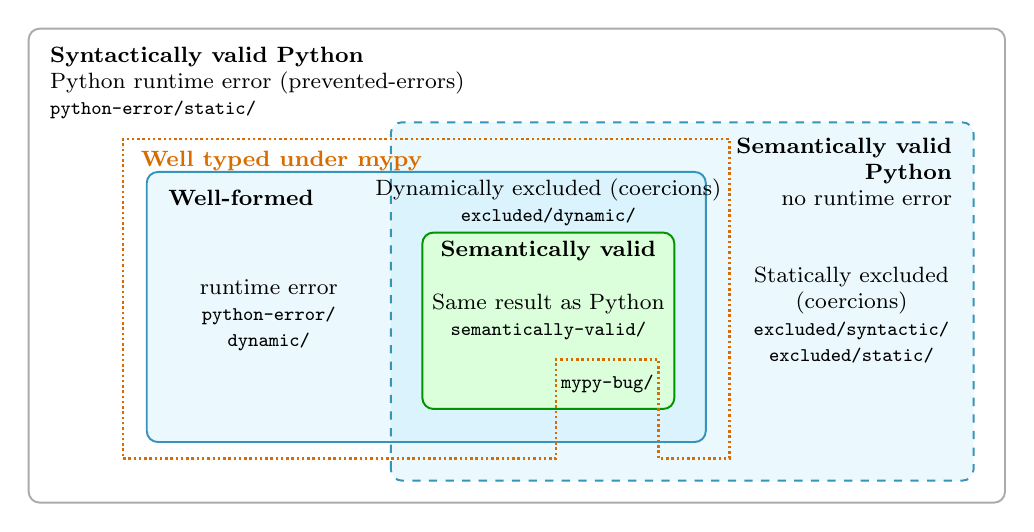
\begin{tikzpicture}[font=\footnotesize, rounded corners=4pt, yscale=0.7]
  \fill[cyan!60, fill opacity=0.13] (4.6,0.4) rectangle (12.0,6.9);
  \fill[cyan!60, fill opacity=0.13] (1.5,1.1) rectangle (8.6,6.0);
  \fill[green!14] (5.0,1.7) rectangle (8.2,4.9);
  \draw[black!33, line width=0.7pt] (0,0) rectangle (12.4,8.6);
  \draw[cyan!72!black, line width=0.7pt] (1.5,1.1) rectangle (8.6,6.0);
  \draw[dashed, cyan!72!black, line width=0.7pt] (4.6,0.4) rectangle (12.0,6.9);
  \draw[green!58!black, line width=0.7pt] (5.0,1.7) rectangle (8.2,4.9);
  \draw[densely dotted, orange!85!black, line width=0.9pt, sharp corners]
    (1.2,0.8) -- (6.7,0.8) -- (6.7,2.6) -- (8.0,2.6) -- (8.0,0.8) -- (8.9,0.8) -- (8.9,6.6) -- (1.2,6.6) -- cycle;
  \node[anchor=north west, align=left] at (0.15,8.45)
    {\textbf{Syntactically valid Python}\\Python runtime error (\figref{prevented-errors})\\\testdir{python-error/static/}};
  \node[anchor=north east, align=right] at (11.85,6.8)
    {\textbf{Semantically valid}\\\textbf{Python}\\no runtime error};
  \node[anchor=north west, text=orange!85!black] at (1.3,6.55) {\textbf{Well typed under mypy}};
  \node[anchor=north west] at (1.65,5.85) {\textbf{Well-formed \PurePy}};
  \node[align=center] at (10.45,3.4)
    {Statically excluded\\(\figref{coercions})\\\testdir{excluded/syntactic/}\\\testdir{excluded/static/}};
  \node[align=center] at (3.05,3.4) {\PurePy runtime error\\\testdir{python-error/}\\\testdir{dynamic/}};
  \node[align=center] at (6.6,5.45) {Dynamically excluded (\figref{coercions})\\\testdir{excluded/dynamic/}};
  \node[align=center] at (6.6,3.85)
    {\textbf{Semantically valid}\\\textbf{\PurePy}\\Same result as Python\\\testdir{semantically-valid/}};
  \node at (7.35,2.15) {\testdir{mypy-bug/}};
\end{tikzpicture}
\caption{Python programs and runs, classified by \PurePy, with test directories}
\label{fig:taxonomy}
\end{figure}


\subsection{Conformance suite}
\label{sec:conformance-suite}

The conformance suite pairs each test with the verdict given by Python itself, and runs on CPython,
GraalPy, and Pyodide. \added{\figref{taxonomy} gives the directory holding the tests of each class of program. Tests of programs which are not syntactically valid Python are in \pyinline{python-error/syntactic/} and \pyinline{python-error/syntactic-only/}.} \todo{Reference interpreter, needed
to detect dynamically excluded operations (\issue{64}).}

